% AAAI 2027 anonymous submission
\documentclass[letterpaper]{article}
\usepackage[submission]{aaai2027}
\usepackage[hyphens]{url}
\usepackage{graphicx}
\urlstyle{rm}
\def\UrlFont{\rm}
\usepackage{natbib}
\usepackage{caption}
\usepackage{amsmath,amssymb,amsfonts}
\usepackage{algorithm}
\usepackage{algorithmic}
\usepackage{booktabs}
\usepackage{multirow}
\frenchspacing

\pdfinfo{/TemplateVersion (2027.1)}
\setcounter{secnumdepth}{0}

\title{ABER: Actuation-Aware Braking-Envelope Recovery\\
for Recursively Safe Robot Learning}
\author{Anonymous Submission}
\affiliations{}

\begin{document}
\maketitle

\begin{abstract}
Safe reinforcement learning must constrain actions a robot can execute, while
avoiding a shield-induced loss of task completion.  We introduce ABER
(Actuation-Aware Braking-Envelope Recovery), a sampled-data shield posed
directly on forward/turn velocity setpoints.  A calibrated stopping envelope
gives a closed-form next-speed cap; the certified branch retains the requested
turn, while an executable $(0,0)$ witness preserves recursive feasibility.
Under trace-testable servo envelopes, we prove collision avoidance for any
finite set of static obstacles and extend the result to measured stopping
envelopes and bounded geometry error.  Strict recovery is safe but can create
long horizon-saturating stalls outside an accepted empirical envelope.  We
therefore introduce ABER-LR, an explicitly uncertified liveness extension
that combines an inflated intervention margin with latched obstacle-relative
restoration until certificate re-entry.  We evaluate the joint endpoint
collision-free success rather than safety or success alone.  Across 30
independently trained policies spanning two training modes and three
Safety-Gymnasium tasks, ABER-LR improves collision-free success over strict
ABER in all six mode--task groups and 28/30 checkpoints.  The checkpoint-level
mean gain is 9.67 points, with collision and timeout reductions of 2.89 and
9.79 points.  Relative to unfiltered execution, collision falls by 38.97
points and collision-free success rises by 3.59 points on average, although
raw success falls and the gain is not universal across tasks.  The results
separate the certified safety layer from empirical safety--liveness
coordination rather than extending the theorem to restoration steps.
\end{abstract}

\section{Introduction}

Reinforcement-learning policies for mobile robots commonly output a normalized
forward/turn command.  The low-level controller holds this command for a finite
period and tracks a translational-speed and turn-rate setpoint.  In contrast,
many safety arguments assume a fully actuated Cartesian acceleration.  This
gap matters most in the fallback branch: projecting a radial acceleration onto
the current heading may neither satisfy the derived constraint nor stop the
vehicle.

We study a sampled state $x_k=(q_k,\theta_k,s_k)$, where $q_k\in\mathbb R^2$
is position, $\theta_k$ is heading, and $s_k\ge0$ bounds translational speed.
The deployed action is $u_k=(u_k^f,u_k^\omega)\in[-1,1]^2$.  Our objective is
not to reintroduce a Cartesian action behind this interface, but to filter the
two motor-level setpoints themselves.

Stopping distance has long appeared in adaptive-cruise CBFs
\cite{ames2014,ames2017}, feasibility analysis
\cite{xiao2022feasibility}, and optimal CBF construction
\cite{beaver2024}.  Sampled-data CBFs explicitly account for zero-order hold
\cite{breeden2022,taylor2022}, zero-order CBFs avoid derivative models
\cite{tan2025}, and collision-cone CBFs encode velocity-obstacle geometry
\cite{tayal2024}.  Therefore, we do not claim
$s^2/(2a_b)$ as new.  The unresolved deployment question is narrower: how can
that reserve yield an action-space projection and a recovery policy that are
both executable by a forward/turn velocity servo, including when several
obstacles are simultaneously active?

ABER answers this question with a scalar next-speed cap.  For clearance
$d$ and sample period $\Delta t$, the largest admissible speed $z$ solves
\begin{equation}
 \Delta t z + \frac{z^2}{2a_b}\le d.                 \label{eq:capineq}
\end{equation}
If the current speed is below the cap, only the forward setpoint is clipped;
the requested turn is retained.  Otherwise the vehicle receives the
zero-speed, zero-turn recovery.  This conservative construction is independent
of obstacle bearing.  That loss of directional permissiveness buys two useful
properties: one recovery protects all static obstacles at once, and the online
work is $O(m)$ for $m$ obstacles without a QP.

The same conservatism creates a second deployment problem.  When the empirical
plant leaves the accepted envelope, repeated $(0,0)$ commands can reduce
collision yet occupy the rest of the task horizon.  We treat this as an
indicator-coordination failure: neither collision nor raw success alone
measures a successful safe completion.  Our empirical extension ABER-LR
couples earlier intervention to a latched obstacle-relative restore, and uses
the joint event $\mathrm{success}\land\neg\mathrm{collision}$ as its primary
endpoint.  Restore is deliberately excluded from the certified witness.

Our contributions are:
\begin{enumerate}
\item an actuation-aware safety-filter design that certifies the executed
sampled-data transition rather than an auxiliary Cartesian input, instantiated
directly in deployed $(\text{forward},\text{turn})$ space: its closed-form
speed cap is maximal within a bearing-independent one-step envelope, is the
unique least-change projection for any positive diagonal action metric, and
costs $O(m)$ for $m$ obstacles without a QP;
\item an executable $(0,0)$ recovery witness and a recursive-feasibility and
collision-avoidance theorem for any finite set of static obstacles, including
explicit closure of the speed bound, a monotone-envelope generalization, and
an uncertainty-inflated certificate; and
\item ABER-LR, an explicitly uncertified liveness extension, and a
falsification-first evaluation that separates certificate validity,
geometric collision, raw success, and collision-free success.  The learned
study uses 30 saved checkpoints and 15,000 matched filter-off/on pairs across
strict ABER and ABER-LR, retaining adverse task and efficiency outcomes.
\end{enumerate}

\section{Related Work}

\textbf{Constraint manifolds and CBFs.}
ATACOM maps policy actions onto a constraint manifold and establishes
continuous-time invariance through null-space dynamics
\cite{liu2022,liu2024,liu2025}.  CBF-QPs similarly modify a nominal command
through an online constrained optimization \cite{ames2017}; HOCBFs treat
higher-relative-degree constraints \cite{xiao2021}.  These are related
projection mechanisms, but a guarantee is tied to the dynamics and action map
used in its derivation.  Our method retains the extended-state manifold view
while replacing a Cartesian tangent cone by a setpoint-level sampled-data
admissible set.

\textbf{Sampling and feasibility.}
Discrete CBFs enforce a one-step condition on a discrete model
\cite{agrawal2017,zeng2021}.  Breeden, Garg, and Panagou derive sufficient
conditions for zero-order-held CBF controllers \cite{breeden2022}, while
Taylor et al. use approximate discrete-time models \cite{taylor2022} and Tan
et al. develop ZOCBFs \cite{tan2025}.  These general frameworks can cover
unicycle systems when appropriate bounds are available.  ABER specializes
the construction to bounded braking: the resulting scalar inverse is closed
form, and feasibility is witnessed by the exact command sent to the robot.

\textbf{Velocity-aware geometry.}
Braking constraints and input compatibility are central in CBF feasibility
\cite{xiao2022feasibility,beaver2024}.  Collision-cone CBFs instead use
relative position and velocity to exclude collision courses
\cite{tayal2024}.  Our certificate is more conservative because it does not
credit a favorable turn or obstacle bearing.  It consequently extends to
multiple static obstacles without requiring intersection feasibility of
directional half-spaces.

\textbf{Safe RL and reachability.}
Safety layers have been combined with policy optimization
\cite{cheng2019,taylor2020}; Lagrangian algorithms enforce expected CMDP costs
rather than per-state invariance \cite{achiam2017,ray2019}.  Hamilton--Jacobi
reachability provides stronger set-based machinery at greater offline cost
\cite{mitchell2005,bansal2017,fisac2019}.  Our optional \emph{sim-BRT} is not
an HJ solve: it is a sampled nine-direction forward rollout used only as a
reward-shaping term.  We therefore report native and shaped training
separately.

\section{Problem Formulation}

\subsection{Executable Action Maps}

Let a nominal policy $\pi$ return $u_{\rm RL}\in[-1,1]^2$ at every sample.
A shield is a map
\begin{equation}
 \Phi:(x_k,u_{{\rm RL},k},\mathcal O)\mapsto u_k,
 \qquad u_k=(u_k^f,u_k^\omega),                       \label{eq:shieldmap}
\end{equation}
where $\mathcal O$ is the finite obstacle description and $u_k$ is the exact
command held by the low-level velocity servo.  Safety must therefore be proved
for the transition relation induced by $u_k$, not for an auxiliary Cartesian
input that is never sent to the plant.  The policy itself is unrestricted: the
certificate must hold for every proposed $u_{\rm RL}$, including actions far
outside the one-step admissible set.

This distinction is structural for nonholonomic platforms.  Write
$e(\theta)=(\cos\theta,\sin\theta)$ and
$e_\perp(\theta)=(-\sin\theta,\cos\theta)$.  For the acceleration-level
unicycle idealization
\begin{equation}
 \dot q=s e(\theta),\qquad \dot s=a,
 \qquad \dot\theta=\omega,                              \label{eq:unicycle}
\end{equation}
the Cartesian acceleration is
$\ddot q=a e(\theta)+s\omega e_\perp(\theta)$.

\textbf{Lemma 1 (Cartesian fallback mismatch).}
At $s=0$, the instantaneous image of every bounded unicycle input
$(a,\omega)$ under (\ref{eq:unicycle}) is the one-dimensional set
$\{a e(\theta)\}$.  Hence a Cartesian safety fallback with nonzero component
along $e_\perp(\theta)$ has no realizing unicycle input at that state.

\textbf{Proof.}
Substituting $s=0$ into $\ddot q$ removes the only lateral term, independently
of $\omega$.  Therefore $e_\perp(\theta)^\top\ddot q=0$ for every admissible
input, which excludes any requested lateral component. $\square$

At $s>0$, the lateral component remains coupled to $s\omega$ and to the turn
bound; it is still not an independent Cartesian degree of freedom.  Lemma~1
does not say that Cartesian CBFs cannot be specialized to unicycles.  It shows
why feasibility in an unconstrained Cartesian action space is insufficient:
the proof must either include the platform action map or, as ABER does, be
posed directly at the deployed interface.

\subsection{Recursive Shield Objective}

For a state set $\mathcal C$, call a shield \emph{recursively feasible} if
every state in $\mathcal C$ admits an action returned by the shield and every
accepted plant transition under that action ends in $\mathcal C$.  This is
stronger than producing a feasible optimization result at the current sample:
it requires the returned action to preserve feasibility of the next sample.
Our goal is a map $\Phi$ satisfying this property for arbitrary nominal policy
actions, while changing the turn request only when the certified recovery
branch is necessary.

The certificate uses path length rather than a bearing-specific radial
velocity.  If a realized trajectory over one sample has length $\ell$, then
for every fixed point $o_i$,
\begin{equation}
 \|q^+-o_i\|\ge \|q-o_i\|-\|q^+-q\|
               \ge \|q-o_i\|-\ell .                    \label{eq:pathlip}
\end{equation}
This bound is independent of heading and is simultaneously valid for every
static obstacle.  It is conservative when the robot turns away, but avoids an
intersection of directional constraints whose feasibility may depend on an
unavailable Cartesian action.

\section{Actuation-Aware Filter}

\subsection{Model and Certificate Interface}

Let static obstacle $i$ have center $o_i$ and keepout radius $r_i$, including
robot body and uncertainty margins.  Define
\begin{equation}
\begin{aligned}
 d_i(q)&=\|q-o_i\|-r_i,\\
 c_i(q,s)&=d_i(q)-D(s), & D(s)&=\frac{s^2}{2a_b},
\end{aligned}                                               \label{eq:manifold}
\end{equation}
where $a_b>0$ is a conservative braking capability and $D$ is a validated
upper bound on stopping path length.  The safe set is
$\mathcal C=\{(q,s):c_i(q,s)\ge0\ \forall i\}$.

The theorem uses a plant acceptance interface rather than a fictitious
acceleration input.  For a held forward/turn setpoint, write $s^+$ for the next
speed and $\ell$ for path length during the interval.  We require:

\textbf{A1 (normal servo envelope).} For a normal action,
\begin{equation}
 s^+\le z:=\max\{s,v_{\max}|u^f|\},\qquad
 \ell\le\Delta t z.                                      \label{eq:normalenv}
\end{equation}

\textbf{A2 (recovery envelope).} The executable command
$u^{\rm rec}=(0,0)$ satisfies
\begin{equation}
 \ell^{\rm rec}+D(s^+)\le D(s).                          \label{eq:recenv}
\end{equation}

Both conditions are directly testable from command, pose, and speed traces.
For the semi-implicit bounded-braking model
$s^+=\max\{s-a_b\Delta t,0\}$ and
$\ell^{\rm rec}\le\Delta t s^+$, (\ref{eq:recenv}) can be checked exactly.
If $s<a_b\Delta t$, both upper bounds are zero.  Otherwise,
\begin{align}
 \ell^{\rm rec}+D(s^+)
 &\le \Delta t(s-a_b\Delta t)
   +\frac{(s-a_b\Delta t)^2}{2a_b}\notag\\
 &=D(s)-\frac12a_b\Delta t^2\le D(s).                  \label{eq:recderive}
\end{align}
Other low-level controllers may use a tabulated stopping envelope $D$; only
its monotonicity and (\ref{eq:recenv}) are needed by the proof.

\subsection{Projection and Recovery}

Let $d_{\min}=\min_i d_i(q)$.  Inverting (\ref{eq:capineq}) gives
\begin{equation}
\begin{aligned}
z_{\max}(d_{\min})=\min\{v_{\max},\;&-a_b\Delta t\\
 &+\sqrt{(a_b\Delta t)^2+2a_bd_{\min}}\},
\end{aligned}                                                   \label{eq:cap}
\end{equation}
with $z_{\max}=0$ when $d_{\min}<0$.  Algorithm~\ref{alg:aber} clips the
forward setpoint when the normal envelope can be certified and otherwise
executes recovery.  Reverse commands are covered through $|u^f|$.

\textbf{Proposition 1 (sharp cap within the envelope).}
For $d\ge0$, let $g(z)=\Delta t z+z^2/(2a_b)$.  Equation~(\ref{eq:cap})
returns
\[
 z_{\max}(d)=\max\{z\in[0,v_{\max}]:g(z)\le d\}.
\]
If $z_{\max}<v_{\max}$, every $z>z_{\max}$ violates the one-step
inequality.  Indeed, $g'(z)=\Delta t+z/a_b>0$ on $z\ge0$, and
(\ref{eq:cap}) is its nonnegative inverse, clipped only at $v_{\max}$.
Thus the cap is not merely sufficient but maximal for the
bearing-independent A1 bound.  This does not claim maximality among
bearing-aware safe actions, which may credit a favorable turn.

The corresponding normal-branch action set is the rectangle
\begin{equation}
 \mathcal U_N(d)=
 \left[-\frac{z_{\max}(d)}{v_{\max}},
        \frac{z_{\max}(d)}{v_{\max}}\right]\times[-1,1]. \label{eq:normalset}
\end{equation}
It is used only when $s\le z_{\max}$; then every $u\in\mathcal U_N$ satisfies
$\max\{s,v_{\max}|u^f|\}\le z_{\max}$.

\textbf{Proposition 2 (least-change interface projection).}
Let $W=\operatorname{diag}(w_f,w_\omega)$ with $w_f,w_\omega>0$.  In the
normal branch, Algorithm~\ref{alg:aber} is the unique solution of
\begin{equation}
 \min_{u\in\mathcal U_N(d_{\min})}
       (u-u_{\rm RL})^\top W(u-u_{\rm RL}).             \label{eq:weightedproj}
\end{equation}
Consequently it is the least-change action for any positive diagonal weighting
of forward and turn commands within the bearing-independent certificate.

\textbf{Proof.}
The objective is strictly convex and the feasible set is a closed convex
rectangle.  The problem separates by coordinate.  Since the turn interval is
the original $[-1,1]$ and $u_{\rm RL}^\omega$ already lies in it, its unique
minimizer is unchanged.  The forward minimizer is the scalar clipping of
$u_{\rm RL}^f$ to the first interval in (\ref{eq:normalset}), exactly as in
Algorithm~\ref{alg:aber}. $\square$

\begin{algorithm}[t]
\caption{ABER forward/turn projection}
\label{alg:aber}
\begin{algorithmic}[1]
\REQUIRE $q,s,u_{\rm RL}$, obstacles, $\Delta t,v_{\max},a_b$
\STATE $d_{\min}\leftarrow\min_i(\|q-o_i\|-r_i)$
\STATE compute $z_{\max}$ by (\ref{eq:cap})
\IF{$s\le z_{\max}$}
  \STATE $u^f\leftarrow\operatorname{clip}(u^f_{\rm RL},-z_{\max}/v_{\max},z_{\max}/v_{\max})$
  \STATE $u^\omega\leftarrow u^\omega_{\rm RL}$
\ELSE
  \STATE $(u^f,u^\omega)\leftarrow(0,0)$ \COMMENT{certified recovery}
\ENDIF
\RETURN $(u^f,u^\omega)$
\end{algorithmic}
\end{algorithm}

\textbf{Theorem 1 (recursive feasibility and safety).}
Let a forward/turn velocity-servo plant satisfy A1--A2, let all obstacles be
static, and let $s_0\le v_{\max}$.  If $(q_0,s_0)\in\mathcal C$, then
Algorithm~\ref{alg:aber} is recursively feasible,
$(q_k,s_k)\in\mathcal C$ for every $k$, $s_k\le v_{\max}$, and no keepout is
entered.  The result holds for any finite number of obstacles.

\textbf{Proof.}
Assume $(q_k,s_k)\in\mathcal C$ and abbreviate $d_{\min}=d_{\min}(q_k)$.
If $s_k\le z_{\max}$, projection gives
$v_{\max}|u_k^f|\le z_{\max}$, hence A1 gives $s_{k+1}\le z_{\max}$ and
$\ell_k\le\Delta t z_{\max}$.  Distance is 1-Lipschitz along path length, so
for every obstacle
\begin{align}
 c_i(q_{k+1},s_{k+1})
 &\ge d_i(q_k)-\ell_k-D(s_{k+1})\\
 &\ge d_{\min}-\Delta t z_{\max}-D(z_{\max})\ge0,        \label{eq:normalproof}
\end{align}
where the last inequality is the definition of the cap.

If $s_k>z_{\max}$, the algorithm issues $(0,0)$.  A2 yields, for every $i$,
\begin{equation}
\begin{aligned}
c_i(q_{k+1},s_{k+1})
 &\ge d_i(q_k)-\ell_k^{\rm rec}-D(s_{k+1})\\
 &\ge d_i(q_k)-D(s_k)=c_i(q_k,s_k)\ge0.
\end{aligned}                                                   \label{eq:recproof}
\end{equation}
Thus both branches preserve the complete intersection, and recovery is a
feasible witness even when directional constraints would conflict.  Finally,
A1 preserves $s\le v_{\max}$ in the normal branch; braking cannot increase it
in recovery.  Induction completes the proof. $\square$

\subsection{General Envelopes and Robust Bounds}

The quadratic $D(s)=s^2/(2a_b)$ gives the closed form in
(\ref{eq:cap}), but the invariance argument is not tied to constant
deceleration.  Let $D:[0,v_{\max}]\to\mathbb R_{\ge0}$ be continuous and
nondecreasing with $D(0)=0$, and define
\begin{equation}
\begin{aligned}
 G_D(z)&=\Delta t z+D(z),\\
 z_D(d)&=\max\{z\in[0,v_{\max}]:G_D(z)\le d\}.
\end{aligned}                                           \label{eq:generalcap}
\end{equation}
For an empty set take $z_D(d)=0$ and enter recovery.  A measured piecewise
linear or tabulated stopping envelope is therefore admissible; when $G_D$ is
strictly increasing, $z_D$ is unique and can be obtained by a scalar monotone
search.  The evaluated ABER implementation retains the quadratic closed form,
so this extension is a scope result rather than a runtime claim for lookup
tables.

\textbf{Theorem 2 (monotone-envelope invariance).}
Replace (\ref{eq:cap}) in Algorithm~\ref{alg:aber} by $z_D(d_{\min})$.
Suppose the normal transition obeys A1 and recovery obeys
$\ell^{\rm rec}+D(s^+)\le D(s)$ for this $D$.  If
$d_i(q_0)-D(s_0)\ge0$ for every static obstacle, then the generalized filter is
recursively feasible and preserves
$d_i(q_k)-D(s_k)\ge0$ for all $i$ and $k$.

\textbf{Proof.}
In the normal branch, $s^+\le z_D$ and $\ell\le\Delta t z_D$.
Monotonicity of $D$ and (\ref{eq:pathlip}) give
\begin{align}
 d_i(q^+)-D(s^+)
 &\ge d_i(q)-\Delta t z_D-D(z_D)\notag\\
 &\ge d_{\min}-G_D(z_D)\ge0.                            \label{eq:generalnormal}
\end{align}
In recovery, (\ref{eq:pathlip}) and the accepted recovery inequality give
\begin{equation}
 d_i(q^+)-D(s^+)\ge d_i(q)-D(s)\ge0.                   \label{eq:generalrec}
\end{equation}
Thus either branch preserves the entire obstacle intersection.  Recovery is
always an available witness on the certified set, and induction proves the
claim. $\square$

The next result turns bounded perception error into the lower-clearance and
upper-speed quantities needed by Theorem~2.  Let $\hat q,\hat o_i,\hat r_i$
be reported robot position, obstacle center, and keepout radius, and assume
\begin{equation}
 \|q-\hat q\|\le\epsilon_q,\quad
 \|o_i-\hat o_i\|\le\epsilon_{o,i},\quad
 r_i\le\hat r_i+\epsilon_{r,i}.                         \label{eq:errorbounds}
\end{equation}
The triangle inequality yields the computable lower bound
\begin{equation}
 \underline d_i=
 \|\hat q-\hat o_i\|-\hat r_i
 -\epsilon_q-\epsilon_{o,i}-\epsilon_{r,i}
 \le d_i(q).                                             \label{eq:lowerclearance}
\end{equation}

\textbf{Corollary 1 (uncertainty-inflated certificate).}
Let $\bar s\ge s$ be a maintained speed upper bound.  Suppose A1--A2 are
validated for the bound-state transition $\bar s\mapsto\bar s^+$, and run the
generalized filter with $\min_i\underline d_i$ and $\bar s$.  If
$\underline d_i(q_0)-D(\bar s_0)\ge0$ for all $i$, then the true clearances
satisfy $d_i(q_k)-D(s_k)\ge0$ for all $i,k$.

\textbf{Proof.}
Equations~(\ref{eq:errorbounds})--(\ref{eq:lowerclearance}) give
$d_i\ge\underline d_i$, while monotonicity gives $D(s)\le D(\bar s)$.
Theorem~2 preserves the stronger surrogate inequalities
$\underline d_i-D(\bar s)\ge0$, which imply the claimed true-state
inequalities. $\square$

This corollary separates statistical estimation from the deterministic safety
argument: confidence bounds or engineering tolerances may supply the
$\epsilon$ values, but the theorem is conditional on those bounds being valid.
Likewise, command latency can be included by validating A1 with an effective
hold period $\Delta t_{\rm eff}$; unmodeled delay is not covered.

\subsection{Necessity and Residual Robustness}

The two terms in $G_D(z)=\Delta t z+D(z)$ play different roles.  The reserve
$D(z)$ pays for stopping after the next sample; $\Delta t z$ pays for motion
during the sample itself.  The following construction shows that the latter
cannot be dropped while retaining a worst-case A1 certificate.

\textbf{Proposition 3 (necessity of sampled displacement).}
Let $D$ be strictly increasing, choose $s\in(0,v_{\max})$, and set
$d=\Delta t s+D(s)$.  Assume the root of $D(z)=d$ lies below $v_{\max}$.
A cap using only $D(z)\le d$ admits $\tilde z=D^{-1}(d)>s$.  There exists an
A1 transition from this certified state whose next certificate is negative.

\textbf{Proof.}
The initial certificate is
$d-D(s)=\Delta t s>0$.  Select an obstacle directly along the realized path
and an A1-admissible transition attaining
$s^+=\tilde z$ and $\ell=\Delta t\tilde z$.  Because
$D(\tilde z)=d$, its next margin is
\begin{equation}
 d-\ell-D(s^+)
 =d-\Delta t\tilde z-D(\tilde z)
 =-\Delta t\tilde z<0.                                 \label{eq:nosamplecounter}
\end{equation}
Thus the truncated cap can cross the certificate before penetrating the
keepout.  In contrast, the full cap has $G_D(s)=d$ and therefore does not
admit a larger speed. $\square$

The recovery branch is also a semantic part of the certificate, rather than
an arbitrary low-speed replacement.  A1 bounds normal commands but does not
require them to begin braking immediately.

\textbf{Proposition 4 (a nonzero fallback is not certified by A1).}
For every $s\in(0,v_{\max}]$ and boundary state $d=D(s)$, there is a
velocity-servo transition relation satisfying A1 for nonzero commands and A2
for $(0,0)$ such that every nonzero fallback leaves the certified set in one
sample.

\textbf{Proof.}
Consider a one-sample setpoint lag: after any nonzero fallback, the plant keeps
$s^+=s$, travels $\ell=\Delta t s$ toward the obstacle, and only then accepts
the new setpoint.  This satisfies A1 because
$s\le\max\{s,v_{\max}|u^f|\}$ and
$\ell\le\Delta t\max\{s,v_{\max}|u^f|\}$.  Its next margin is
\begin{equation}
 d-\ell-D(s^+)=D(s)-\Delta t s-D(s)=-\Delta t s<0.
                                                               \label{eq:noreccounter}
\end{equation}
Define the response to the exact command $(0,0)$ instead by any braking
transition satisfying A2, such as (\ref{eq:recderive}).  That command preserves
the boundary by Theorem~1, while the nonzero fallback does not. $\square$

Propositions~3--4 are worst-case statements about the accepted interface, not
claims that every physical servo attains the adversarial transitions.  They
explain why the component study tests certificate margin at the constructed
boundaries $d=\Delta t s+D(s)$ and $d=D(s)$, rather than relying only on
observed collision.  They also delimit the claim: a nonzero recovery could be
used if its own trace envelope replaced A2 and were proved to preserve the
reserve.

Trace calibration may leave bounded normal-branch residuals.  Suppose a
validation procedure establishes, for constants
$\varepsilon_s,\varepsilon_\ell\ge0$,
\begin{equation}
 s^+\le z+\varepsilon_s,
 \qquad \ell\le\Delta t z+\varepsilon_\ell,             \label{eq:residualenv}
\end{equation}
where $z=\max\{s,v_{\max}|u^f|\}$ and $D$ is defined through
$v_{\max}+\varepsilon_s$.  Define the tightened cap
\begin{equation}
\begin{aligned}
 z_{D,\varepsilon}(d)=\max\bigl\{z\in[0,v_{\max}]:\ &
 \Delta t z+\varepsilon_\ell\\
 &+D(z+\varepsilon_s)\le d\bigr\}.
\end{aligned}                                           \label{eq:robustcap}
\end{equation}
If the set is empty, ABER enters recovery.

\textbf{Proposition 5 (residual-robust normal branch).}
Under (\ref{eq:residualenv}), replacing $z_D$ by
$z_{D,\varepsilon}$ makes every accepted normal transition preserve all
obstacle certificates.  If the unchanged recovery branch satisfies A2, the
recursive conclusion of Theorem~2 follows.

\textbf{Proof.}
For every obstacle, monotonicity of $D$, (\ref{eq:pathlip}), and the tightened
cap give
\begin{align}
 d_i(q^+)-D(s^+)
 &\ge d_i(q)-\Delta t z-\varepsilon_\ell
                 -D(z+\varepsilon_s)\notag\\
 &\ge d_{\min}-\Delta t z-\varepsilon_\ell
                 -D(z+\varepsilon_s)\ge0.              \label{eq:residualproof}
\end{align}
The recovery step is unchanged, so the same induction applies. $\square$

For the quadratic reserve, (\ref{eq:robustcap}) remains a scalar quadratic
inequality and therefore retains a closed-form positive root.  Setting both
residuals to zero recovers (\ref{eq:cap}).  Additive errors are not silently
absorbed into an empirical claim: they must be predeclared from trace bounds,
and a platform whose residuals exceed them is outside the certificate.

With lower clearances already computed, finding their minimum takes $O(m)$
time and $O(1)$ streaming memory, while all remaining quadratic-envelope
operations are constant time.  Hence the multi-obstacle guarantee does not
conceal an online optimization problem.

\subsection{Regularity and Obstacle Composition}

Besides being closed form, the quadratic cap has useful regularity.  Before
the $v_{\max}$ saturation, implicit differentiation of
$\Delta t z+D(z)=d$ gives
\begin{equation}
 \frac{\mathrm d z_{\max}}{\mathrm d d}
 =\frac{a_b}{\sqrt{(a_b\Delta t)^2+2a_bd}}
 =\frac{1}{\Delta t+z_{\max}/a_b},                     \label{eq:capderivative}
\end{equation}
and
\begin{equation}
 \frac{\mathrm d^2 z_{\max}}{\mathrm d d^2}
 =-\frac{a_b^2}{\bigl((a_b\Delta t)^2+2a_bd\bigr)^{3/2}}<0. \label{eq:capconcavity}
\end{equation}
Thus $z_{\max}$ is nondecreasing and concave in clearance.  Since the first
derivative is at most $1/\Delta t$, saturation at $v_{\max}$ preserves the
global bound
\begin{equation}
 |z_{\max}(d_1)-z_{\max}(d_2)|
 \le\frac{|d_1-d_2|}{\Delta t},
 \qquad d_1,d_2\ge0.                                    \label{eq:caplipschitz}
\end{equation}
This bound is descriptive of the cap, not a substitute for the one-sided
uncertainty treatment in Corollary~1: using a noisy clearance without a valid
lower bound can still overestimate safety.

\textbf{Proposition 6 (normal-projection sensitivity).}
Let $P_d(a)=\operatorname{clip}(a,-z_{\max}(d)/v_{\max},
z_{\max}(d)/v_{\max})$.  For any $a_1,a_2\in[-1,1]$ and
$d_1,d_2\ge0$,
\begin{equation}
 |P_{d_1}(a_1)-P_{d_2}(a_2)|
 \le |a_1-a_2|+
 \frac{|d_1-d_2|}{v_{\max}\Delta t}.                  \label{eq:projsensitivity}
\end{equation}

\textbf{Proof.}
For fixed $d$, scalar projection onto a closed interval is nonexpansive, so
$|P_d(a_1)-P_d(a_2)|\le|a_1-a_2|$.  For fixed $a$, changing the symmetric
interval radius changes the clipped value by no more than the change in that
radius.  Apply the triangle inequality and (\ref{eq:caplipschitz}). $\square$

Therefore the normal-branch forward action is continuous in both nominal
forward command and certified clearance, and the turn action is exactly the
nominal turn.  The complete shield need not be continuous at
$s=z_{\max}(d)$ because crossing that surface activates the discrete recovery
$(0,0)$.  This is an intentional safety switch; the theorem does not claim
smoothness or absence of chattering at that boundary.

For multiple obstacles, the scalar reduction itself adds no conservatism
beyond the bearing-independent path envelope.  Indeed, because $G_D$ is
common to all obstacles,
\begin{equation}
 \bigl[G_D(z)\le d_i\ \forall i\bigr]
 \quad\Longleftrightarrow\quad
 G_D(z)\le\min_i d_i.                                   \label{eq:minexact}
\end{equation}

\textbf{Proposition 7 (monotone obstacle composition).}
For a finite obstacle set $\mathcal O$, the generalized cap satisfies
\begin{equation}
 z_D\!\left(\min_{i\in\mathcal O}d_i\right)
 =\min_{i\in\mathcal O} z_D(d_i).                      \label{eq:capcomposition}
\end{equation}
If $\mathcal O\subseteq\mathcal O'$, then the cap for $\mathcal O'$ cannot
exceed that for $\mathcal O$.  Hence adding an obstacle cannot enlarge the
certified normal-action set, while the same recovery witness continues to
preserve the complete intersection.

\textbf{Proof.}
Equation~(\ref{eq:minexact}) shows that the feasible scalar-speed set for all
obstacles is exactly the intersection of their individual feasible intervals.
Each interval begins at zero, so the endpoint of the intersection is the
minimum of the individual endpoints.  Set inclusion gives the monotonicity
claim, and Theorem~2 gives recovery feasibility. $\square$

\textbf{Proposition 8 (inter-sample keepout avoidance).}
Under the assumptions of Theorem~1, the certificate prevents keepout entry
throughout each held control interval, not only at its endpoints.

\textbf{Proof.}
Let $q(\tau)$ be any intermediate configuration and let $\ell(\tau)$ be the
path length accumulated since $q_k$.  The distance-to-set map is
1-Lipschitz, so
$d_i(q(\tau))\ge d_i(q_k)-\ell(\tau)$ for every obstacle.  On the normal
branch, $\ell(\tau)\le\ell_k\le\Delta t z_{\max}$ and
$d_i(q_k)\ge\Delta t z_{\max}+D(z_{\max})$; hence
$d_i(q(\tau))\ge D(z_{\max})\ge0$.  On the recovery branch,
$\ell(\tau)\le\ell_k^{\rm rec}$ and A2 gives
$\ell_k^{\rm rec}+D(s_{k+1})\le D(s_k)$.  Since
$d_i(q_k)\ge D(s_k)$, it follows that
$d_i(q(\tau))\ge D(s_{k+1})\ge0$.  Thus neither branch can cross a declared
static keepout between samples. $\square$

\subsection{Liveness-Aware Empirical Recovery}

Strict ABER uses $(0,0)$ because A2 makes it a common witness for every
static obstacle.  In Safety-Gym, however, an uncertified robot can approach
zero speed without re-entering $\mathcal C$; repeating the witness then
creates a recovery tail rather than task progress.  ABER-LR addresses this
empirical failure without modifying Algorithm~\ref{alg:aber} or Theorem~1.

Let $j$ index the minimum-clearance obstacle and let
$n=(q-o_j)/\|q-o_j\|$ point away from it.  Resolving $n$ in the body frame
gives $n_f=e(\theta)^\top n$ and
$n_\perp=e_\perp(\theta)^\top n$.  When the inflated certificate is negative
and $s\le s_{\rm stop}$, ABER-LR starts the bounded restore
\begin{equation}
 u^{\rm LR}=\bigl(\operatorname{clip}(\alpha n_f,-\alpha,\alpha),
 \operatorname{clip}(\kappa n_\perp,-1,1)\bigr),       \label{eq:lrrestore}
\end{equation}
with a small nonzero translation floor to avoid yaw-only stalling.  The
restore is latched until certificate re-entry; without the latch, one restore
step raises speed and the next step returns to hard braking.  Experiments fix
$s_{\rm stop}=0.05$, $\alpha=0.25$, $\kappa=1$, $a_b=0.9$, and an inflated
0.10-m margin before cross-task evaluation.

Equation~(\ref{eq:lrrestore}) is an empirical outer recovery controller, not
an A2 witness.  Its steps are marked uncertified, and every theorem and
certificate count below refers only to strict ABER under the accepted plant
interface.  This separation lets us test whether liveness can be recovered
without retroactively labeling the fallback as safe.

\textbf{Scope and deployment.}
A1--A2 are trace-testable plant contracts, not consequences of sending a low
setpoint.  Deployment requires measuring the effective hold period, fitting a
conservative $D$, validating normal and recovery traces, and inflating geometry
as in Corollary~1.  Moving obstacles, unmatched delay, starts outside
$\mathcal C$, or a platform that fails either trace test are not covered.

\section{Experiments}

We test component necessity, safety and task completion on the accepted
interface, learned-policy behavior outside a globally accepted envelope, and
reproducibility.  Protocols, seeds, metrics, and failures are fixed before
aggregation; certificate violations, geometric collisions, and Safety-Gym
costs are reported separately because they are not interchangeable.

\subsection{Falsification-First Component Study}

We first test the two algorithmic branches and the calibration premise rather
than infer them from a collision count.  The grid crosses
$\Delta t\in\{0.02,0.05,0.10,0.20\}$~s, actual-to-configured braking ratio
$\rho\in\{0.5,0.75,1.0,1.25\}$, and $m\in\{1,4,8\}$ obstacles.  We compare
full ABER with (i)~a cap that omits $\Delta t z$, and (ii)~a variant that
keeps the cap but clips to a nonzero setpoint instead of issuing $(0,0)$ when
$s>z_{\max}$.  Every cell uses 1,000 one-step samples for each of two
predeclared boundary challenges and 50 seeded navigation episodes.

The sampled-term challenge starts at $d=\Delta t s+D(s)$, where full ABER is
exactly feasible but the shortened cap can over-accelerate.  The recovery
challenge starts at $d=D(s)$, where A2 certifies $(0,0)$ but does not certify
a nonzero lower setpoint.  These constructed trials test the recursive
certificate before physical penetration; collision is a secondary endpoint.

\begin{table}[t]
\centering
\small
\setlength{\tabcolsep}{3.0pt}
\begin{tabular}{lrrrr}
\toprule
Navigation condition & Epis. & Viol. & Coll. & Succ.\\
\midrule
Full ABER, $\rho\ge1$ & 1200 & 0 & 0 & 1186\\
No sampled term, $\rho\ge1$ & 1200 & 1200 & 481 & 719\\
No recovery, $\rho\ge1$ & 1200 & 1002 & 298 & 902\\
Full ABER, $\rho<1$ & 1200 & 873 & 539 & 660\\
\bottomrule
\end{tabular}
\caption{Component navigation study.  ``Viol.'' counts episodes that leave
the braking-envelope certificate; ``Coll.'' counts keepout entry.  The 14
calibrated full-ABER nonsuccesses are horizon timeouts, not collisions.}
\label{tab:ablation}
\end{table}

In the calibrated boundary controls, full ABER has 0/24,000 violations on
each challenge.  Omitting the sampled term causes 24,000/24,000 violations on
its challenge; omitting recovery does the same on the recovery challenge.
With $\rho<1$, even full ABER violates 24,000/24,000 recovery challenges, as
expected when A2 is false.  Table~\ref{tab:ablation} shows that the same
distinctions persist in navigation: both ablations sometimes make more
short-term progress, but only by leaving the certified set.

The complete artifact contains 288,000 boundary records and 7,200 navigation
records.  All 48 predeclared grid checks pass, and two formal runs produce the
same raw SHA-256.  Thus the experiment supports necessity within the stated
A1--A2 interface; it does not claim that every velocity servo exhibits the
particular one-sample nonzero-setpoint delay used to expose the distinction.

\subsection{Certified-Envelope Comparison}

We first evaluate exactly the plant used by Theorem~1.  Parameters are
$\Delta t=0.1$~s, $v_{\max}=1$~m/s, $a_b=a_{\rm acc}=0.9$~m/s$^2$,
$|\omega|\le1.5$~rad/s, and $r_i=0.25$~m.  A shared reactive navigator
produces the nominal forward/turn action.  We sample 100 single-obstacle and
100 four-obstacle layouts from fixed seeds, all starting at rest in
$\mathcal C$.  Baselines are fixed geometry-specialized implementations of a
continuous braking-distance CBF, a one-step sampled-data CBF/ZOCBF, and a
collision-cone CBF; this benchmark does not claim to reproduce every tuning
choice in their source papers.  Raw per-episode results and the complete
manifest are included with the submission.

\begin{table}[t]
\centering
\small
\setlength{\tabcolsep}{2.5pt}
\begin{tabular}{llrrrr}
\toprule
Scene & Method & Coll. & Succ. & Time & min clr.\\
 & & (\%) & (\%) & (s) & worst (m)\\
\midrule
\multirow{4}{*}{Single}
 & Braking CBF & 0 & 100 & 5.80 & 0.290\\
 & SD-CBF/ZOCBF & 0 & 100 & \textbf{4.90} & 0.185\\
 & Collision cone & 0 & 100 & 5.91 & 0.083\\
 & \textbf{ABER} & 0 & 100 & 6.46 & 0.016\\
\midrule
\multirow{4}{*}{Multi}
 & Braking CBF & 0 & 100 & 7.22 & 0.220\\
 & SD-CBF/ZOCBF & 0 & 100 & \textbf{5.55} & 0.046\\
 & Collision cone & 0 & 100 & 7.33 & 0.001\\
 & \textbf{ABER} & 0 & 100 & 7.22 & 0.016\\
\bottomrule
\end{tabular}
\caption{Fixed-config certificate-envelope results (100 episodes per cell).
All methods are safe here; only ABER is evaluated against Theorem~1 and has
zero certificate violations in both scenes.  Minimum clearance is relative to
the declared keepout.}
\label{tab:cert}
\end{table}

Table~\ref{tab:cert} does not support a claim that other filters are unsafe.
It shows instead that ABER's formal guarantee is obtained without stopping
the task: all ABER trials reach the goal.  It is slower in the single
obstacle case and essentially matches braking CBF time in the multi-obstacle
case.  Its smaller clearance is expected because the cap uses available
stopping reserve rather than a directional stand-off.

\begin{figure*}[t]
  \centering
  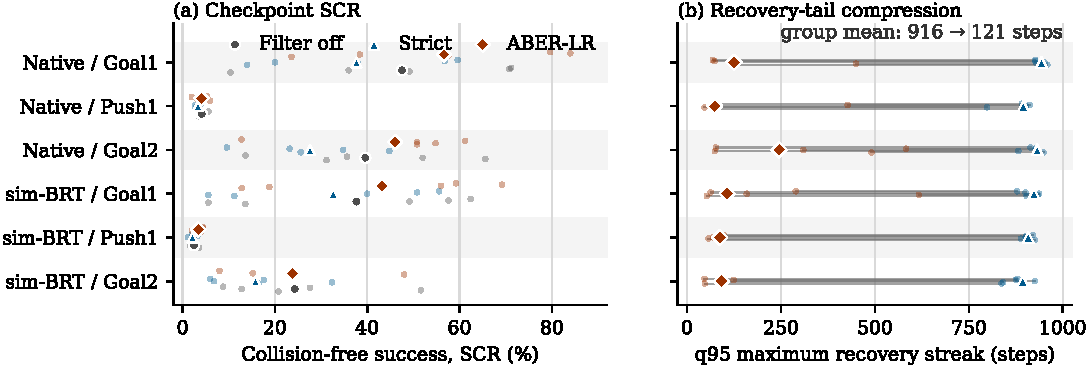
\includegraphics[width=0.98\textwidth]{../figures/main/aber_lr_full_matrix.pdf}
  \caption{Frozen 30-checkpoint study.  Small symbols are checkpoints and
  large symbols are group means.  (a)~Collision-free success.
  (b)~Same-checkpoint strict-to-LR q95 recovery-tail contraction (gray links).}
  \label{fig:aber-lr-matrix}
\end{figure*}

\subsection{Learned-Policy Studies}

We next use Safety-Gymnasium Point Goal1, Push1, and Goal2
\cite{ji2023}.  Source inspection gives an environment period of
$10\times0.002=0.02$~s.  Twenty zero-setpoint braking traces measured a peak
speed of 1.468~m/s and a minimum stopping-path equivalent deceleration of
2.06~m/s$^2$; we use the conservative envelope
$v_{\max}=1.5$~m/s and $a_b=0.9$~m/s$^2$.  These are empirical plant
acceptance measurements, not evidence that MuJoCo satisfies A1--A2 globally.

Each setting uses PPO for 200K steps and five seeds.  Native training is
compared with sim-BRT reward shaping, a five-step forward rollout rather than
HJ reachability.  The supplement retains the unpaired integration matrix; the
intervention claim uses the matched execution toggle below.
\paragraph{Paired safety--liveness isolation.}
We save all 30 policies in the two-mode, three-task, five-seed matrix.  Each
checkpoint is evaluated with deterministic actions on 250 predeclared reset
seeds under filter-off, strict ABER, and the parameter-frozen ABER-LR.
Strict and LR runs use identical checkpoints and initial snapshots; their
independently rerun filter-off records agree exactly.  This yields 7,500
matched pairs per filtered variant.  The generalization unit is the trained
checkpoint; episode pairing controls reset variation, and confidence
intervals resample checkpoints.

Raw success can count an episode that also collides.  We therefore define
safe completion as
\begin{equation}
 \mathrm{SCR}=\Pr(\mathrm{success}\land
                    \neg\mathrm{geometric\ collision}),       \label{eq:scr}
\end{equation}
and report it with both marginals, unsafe success, and timeout.  This joint
event introduces no tuned scalarization weight.

Negative tests are classified by the failed gate: collision (safety), success
or recovery tail (liveness), SCR (coordination), or consistency across seeds
and tasks (transfer).  The supplement retains every rejected recovery pilot.

\begin{table}[t]
\centering
\small
\setlength{\tabcolsep}{2.6pt}
\begin{tabular}{lrrrrr}
\toprule
Execution & Succ. & Coll. & SCR & Unsafe succ. & Timeout\\
\midrule
Filter off & 42.48 & 43.19 & 25.96 & 16.52 & 57.52\\
Strict ABER & 19.92 & 7.11 & 19.88 & \textbf{0.04} & 80.08\\
ABER-LR & 29.71 & \textbf{4.21} & \textbf{29.55} & 0.16 & \textbf{70.29}\\
\bottomrule
\end{tabular}
\caption{Equal-weight 30-checkpoint learned-policy summary (\%).  SCR is
$\Pr(\mathrm{success}\land\neg\mathrm{geometric\ collision})$; unsafe
success is the complementary successful-but-colliding event.}
\label{tab:aber-lr-summary}
\end{table}


Relative to strict ABER, ABER-LR increases checkpoint-level SCR by
9.67 points (checkpoint bootstrap 95\% CI $[6.37,13.33]$), success by
9.79 points, and reduces collision and timeout by 2.89 and 9.79 points.
All six mode--task means and 28/30 checkpoints improve SCR
(Fig.~\ref{fig:aber-lr-matrix}).  A gate frozen before cross-task
transfer---success gain at least 10 points, no collision increase, SCR gain at
least 5 points, and SCR improvement in at least four seeds---passes for Native Goal1, Native Goal2,
and sim-BRT Goal1.  sim-BRT Goal2 improves SCR in 5/5 seeds but misses the
10-point success threshold; both Push1 policies have only 4.6--5.1\%
unfiltered success, limiting the absolute completion gain.

Relative to filter-off execution, ABER-LR lowers collision by 38.97 points
and unsafe success by 16.36 points.  Mean SCR rises by 3.59 points
($[1.03,6.37]$), but raw success falls by 12.77 points and timeout rises by
the same amount.  Moreover, SCR improves in only four of six group means and
17/30 checkpoints.  Thus the evidence supports indicator coordination on
average, not universal dominance over the unfiltered policy.

The mechanism matches the hypothesis: mean recovery occupancy falls from
51.15\% to 22.76\%, the group-average q95 streak from 916 to 121 steps, and
timeout by 9.79 points.  In an earlier 250-pair pilot, yaw-only escape left
q95 at 958 and gained only 1.6 success points; $a_b=1.5/2.0$ left q95 above
960 and reduced success.  Exit authority, not only recovery entry, is the
difficulty.  This is liveness evidence, not a restore certificate.
\section{Limitations and Conclusion}

Strict ABER assumes an accepted static-obstacle envelope and certified start;
Safety-Gym and LR restore remain empirical, and Push1 contacts lie outside the
theorem.  ABER certifies the transition caused by the executed action;
ABER-LR coordinates that conservative witness with liveness, improving
collision-free completion over strict ABER in all six groups without extending
the theorem to restoration.  A directional-restore certificate under measured
servo dynamics remains open; LR evidence is empirical.  Rejected variants
therefore define the mechanism boundary, rather than hidden tuning runs.

\bibliography{references}
\end{document}
